%%%%%%%%%%%%%%%%%%%%%%%%%%%%%%%%%%%%%%%%%%%%%%%%%%%%%%%%%%%%%%%%%%%%%%%%
% Preamble
%%%%%%%%%%%%%%%%%%%%%%%%%%%%%%%%%%%%%%%%%%%%%%%%%%%%%%%%%%%%%%%%%%%%%%%%
\documentclass[11pt]{article}
%
% Packages and other includes
% Pagination
\usepackage[letterpaper, margin=1in]{geometry}
\usepackage{emptypage}
\usepackage[backend=biber,style=chem-acs]{biblatex}
\addbibresource{references.bib}
\usepackage{ulem}
\usepackage{xcolor}
%
% Fonts
\usepackage[T1]{fontenc} % best for Western European languages
\usepackage{lmodern} % Latin Modern instead of CM
\usepackage{textcomp} % required to get special symbols
%
% Math
\usepackage{amsmath, amssymb}
\usepackage{braket}
%
% Graphics, floats, tables
\usepackage{graphicx, color, float, array}
%
% Hyperlinks
\usepackage{hyperref}
%
%
% Definitions and settings
% Paragraph indent and spacing
\setlength{\parskip}{0.4\baselineskip}
\setlength{\parindent}{0in}
%
%
% Title, authors, date
\title{\textbf{Worksheet 5}}
\date{\vspace{-2em}February 2nd, 2022}
%
%
%%%%%%%%%%%%%%%%%%%%%%%%%%%%%%%%%%%%%%%%%%%%%%%%%%%%%%%%%%%%%%%%%%%%%%%%
% Main document
%%%%%%%%%%%%%%%%%%%%%%%%%%%%%%%%%%%%%%%%%%%%%%%%%%%%%%%%%%%%%%%%%%%%%%%%
%

\begin{document}

\maketitle

Collaborations are encouraged and students must report all collaborators
on each assignment. All external sources (websites, books) must be
cited. An \textit{extra credit} (\textit{EC}) problem will be available per
assignment. Please submit a completed homework on-time to receive \textit{EC}
and no partial \textit{EC} (all parts must be correct) will be given out.
Additional problems are listed at the end of each assignment. This week's
assignment is due \textit{Tuesday, Feb 8th at 10:00am.}

\textbf{Enthalpy $\Delta H$, Entropy $\Delta S$, and Free Energy $\Delta G$}

1. (2 pts) Determine $\Delta S_\text{sys}$, $\Delta S_\text{surr}$, and $\Delta S_\text{tot}$ for the
following process of 1.48 mols of ideal gas molecules from 13.17 atm to 0.447 atm
and 1.29 L at 350K. Report results to 3 significant figures.

(a) A reversible isothermal expansion

(b) An isothermal irreversible free expansion

\vspace{2.5in}

2. (2 pts) Determine the change in entropy if 2 gallons of water at $93^\circ\text{C}$ is added to
1.25 gal of water at $25^\circ\text{C}$. Report results to 3 significant figures.

\vspace{2.5in}

3. (4 pts) Diethyl zinc is a highly reactive compound when it comes into contact with oxygen molecules
to form zinc oxide, carbon dioxide, and water at 298K. Determine the following and report results
to 3 significant figures.

(a) Write a balanced chemical equation including states.

(b) Calculate the enthalpy of reaction and entropy change.

(c) Determine whether this reaction is exothermic or endothermic. Is this reaction spontaneous
at room temperatue?

\vspace{2.5in}

4. (4 pts) Acetic acid, CH$_3$COOH(l), could be produced from the reactions of methanol with carbon monoxide,
the oxidation of ethanol, or the reaction of carbon dioxide with methane.

(a) Write balanced chemical equations including states for each process.

(b) Compute the enthalpy of reaction and change in entropy for each process. Report the results
to 4 significant figures.

(c) Determine which process would be the easiest to produce acetic acid. Justify your choice.

\pagebreak

%5. The protein lysozyme unfolds at a transition temperature of $75.5^\circ\text{C}$ and the
%standard enthalpy of transition is $509 \text{kJ/mol}$. Calculate the entropy of unfolding
%of lysozyme at $25.0^\circ\text{C}$, given that the difference in the constant-pressure
%heat capacities upon unfoldin is $6.28 \text{kJ/mol}$ and can be assume to be independent
%of temperature. \textit{Hint:} Imagine that the transition at $25.0^\circ\text{C}$ occurs
%in three steps. (i) heating of the folded protein from $25.0^\circ\text{C}$ to the transition
%temperature, (ii) unfolding at the transiton temperature, and (iii) cooling of the unfolded
%protein to $25.0^\circ\text{C}$.
%
%\pagebreak

5. (8 pts) \textbf{Carnot Cycle} The steam engine played an important role during the industrial
revolution. A French engineer Nicolas L\'{e}onard Sadi Carnot investigated the efficiency
of the heat engine. For an ideal gas, he developed the most efficient engine known as the Carnot cycle, see
Fig. \ref{fig:carnot}. The cycle consists of four processes: (i) Reversible isothermal expansion,
(ii)Reversible adiabatic expansion, (iii) Reversible isothermal compression, and (iv) Reversible
adiabatic compression.

(a) Determine the heat $Q$, the work $W$, the entropy $\Delta S$, and the internal energy $\Delta U$
at each step of the Carnot cylce. Define all variables.

(b) What is the total $W$, $Q$, $\Delta S$, and $\Delta U$ for 1 cycle ($1\rightarrow 2 \rightarrow 3
\rightarrow 4 \rightarrow 1$)?

(c) Using part b), calculate the efficiency of this engine.

(d) You are operating a Carnot engine with a heat reservoir of 500K and heat sink of
298K. What is the efficiency of your engine?

\begin{figure}[hbpt]
  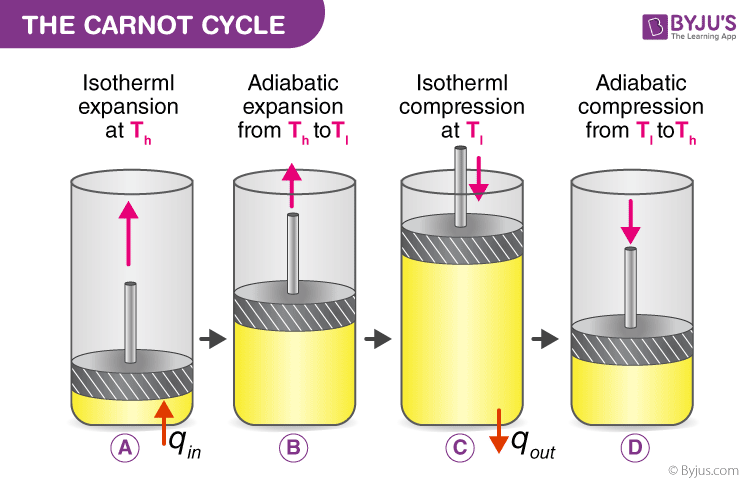
\includegraphics[width=0.45\textwidth]{carnot.png}
  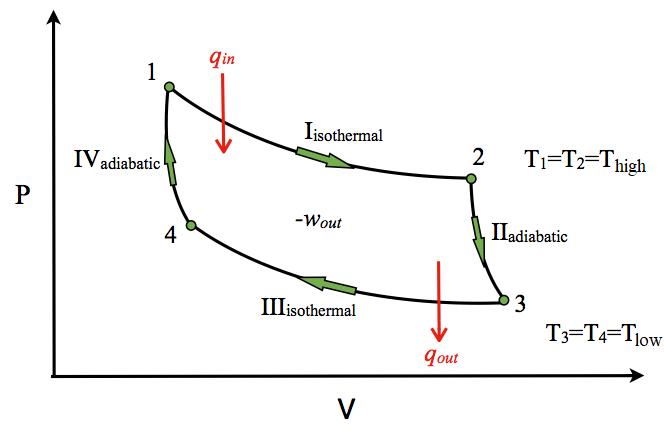
\includegraphics[width=0.5\textwidth]{pv_carnot.png}
  \caption{Illustration of the carnot cycle and PV diagram.}
  \label{fig:carnot}
\end{figure}

\pagebreak

\textbf{Gibbs Free Energy}

6. (7 pts) \textit{Extra Credit:} In biology, biochemical processes are often unfavorable and
requires coupling them to a favorable reaction. For example, adenosine triphosphate (ATP) is
the primary energy source for living cells and drives vital nonspontaneous chemical reactions.
However, the formation of ATP is an unfavorable process. Cells use oxidative phosphorylation
to generate ATP at pH = 7:
\begin{enumerate}
\item ADP$^{3-}$(aq) + HPO$^{2-}_4$(aq) + H$^+$(aq) $\rightarrow$ ATP$^{4-}$(aq) +H$_2$O(l)
  \hfill $\Delta G = +30.5 \text{kJ}$
\item NADH(aq) $\rightarrow$ NAD$^+$(aq) + H$^+$(aq) + 2 e$^-$
  \hfill $\Delta G = -158.3 \text{kJ}$
\item $\frac{1}{2}$ O$_2$(g) + 2 H$^+$(aq) + 2 e$^-$ $\rightarrow$ H$_2$O(l)
  \hfill $\,\Delta G = -61.9 \text{kJ}$
\end{enumerate}

Report all results to 3 significant figures.

(a) The oxidative phosphorylation is highly efficient.\autocite{Wikstrom2020} Assuming 90$\%$
efficiency, what amount (in moles) of ATP could be formed if 4.50 mol NADH were used to
generate ATP?

(b) Since only $90\%$ of the energy goes into synthesizing ATP, what happened to the remaining
energy? 

(c) In bacteria, acetyl phosphate plays an important role to regulate metabolic functions.
When there is a lack of acetate, bacteria hydrolyze acetyl phosphate to release acetate
and continue the Kreb Cycle. This reaction has $\Delta G = -41 \text{kJ/mol}$ at pH = 7. To
replenish acetyl phosphate, what is the minimum amount of ATP molcules (in moles) that would
have to be hydrolyzed to form 1.37 mol acetyl phosphate molecules by phosphorylation of acetic acid?

%2. \textbf{Born--Haber Cycle} (6 pts) Ionic solids are extremely stable and lattice energy
%is an additional energy contribution to the overall stability. However, the lattice
%energy cannot be measured directly. The Born--Haber cycle uses the Hess's Law and allows us
%to compute the lattice energies of an ionic compound. The cycle is sketched for NaCl,
%\begin{center}
%  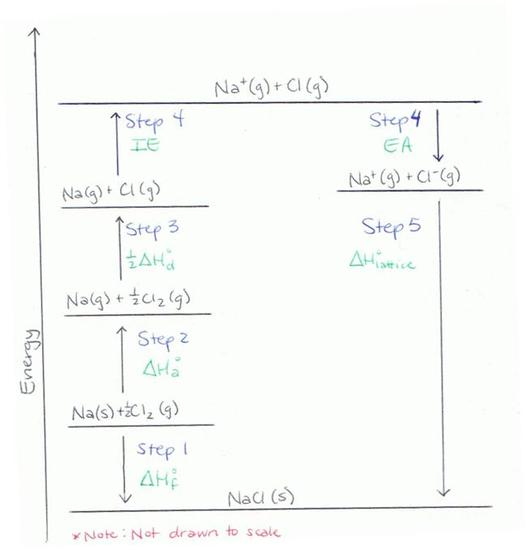
\includegraphics[scale=0.5]{born_haber_nacl.jpg}
%\end{center}
%
%This involves sublimation energy, dissociation energy, ionization energy,
%and electron affinity. The sum of these processes yields the lattice energy. Repeat
%this for cesium oxide (Cs$_2$O).
%
%(a) Draw the Born--Haber cycle.
%
%(b) Look up the enthalpy for the various processes (remember to cite) and calculate
%the lattice energy of Cs$_2$O. Write all thermochemical equations for each step.

%Atkins 8.35

%3. (4 pts) Without performing any calculations, predict whether there is an increase or
%decrease in entropy for each of the following processes:
%
%(a) Cl$_2$(g) + H$_2$O(l) $\rightarrow$ HCl(aq) + HClO(aq)
%
%(b) SO$_2$(g) + Br$_2$(g) + 2 H$_2$O(l) $\rightarrow$ H$_2$SO$_4$(aq) + 2 HBr(aq)
%
%(c) NaCl(s) $\rightarrow$ NaCl(aq)
%
%(d) Cu$_3$(PO$_4$)$_2$(s) $\rightarrow$ 3 Cu$^{2+}$(aq) + 2 PO$_4^{3-}$(aq)
%
%\vspace{1in}
%
%4. The following is a molecular visulization of a system undergoing a spontaneous
%change. Determine from the picture whether entropy increases or decreases during the
%process. Account for the spontaneity of the process in terms of the entropy changes
%in the system and the surroundings. The therometers show the temperature of the
%system.
%
%\begin{center}
%  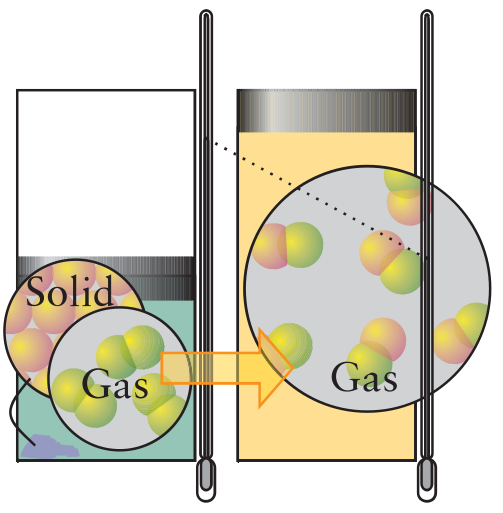
\includegraphics[scale=0.33]{entropy.png}
%\end{center}


\vfill
\textbf{Optional Additional Problems:} Ch. 18 - odd problems 43 - 67

\end{document}
